%%% Econ711: Microeconomics I
%%% Fall 2020
%%% Danny Edgel
%%%
% Due on Canvas Monday, November 30, 11:59pm Central Time
%%%

%%%
%							PREAMBLE
%%%

\documentclass{article}

%%% declare packages
\usepackage{amsmath}
\usepackage{amssymb}
\usepackage{array}
\usepackage{bm}
\usepackage{changepage}
\usepackage{centernot}
\usepackage{graphicx}
\usepackage{multirow}
\usepackage[shortlabels]{enumitem}
\usepackage{fancyhdr}
	\fancyhf{} % sets both header and footer to nothing
	\renewcommand{\headrulewidth}{0pt}
    \rfoot{Edgel, \thepage}
    \pagestyle{fancy}
	
%%% define shortcuts for set notation
\newcommand{\N}{\mathbb{N}}
\newcommand{\Z}{\mathbb{Z}}
\newcommand{\R}{\mathbb{R}}
\newcommand{\Q}{\mathbb{Q}}
\newcommand{\lmt}{\underset{x\rightarrow\infty}{\text{lim }}}
\newcommand{\neglmt}{\underset{x\rightarrow-\infty}{\text{lim }}}
\newcommand{\zerolmt}{\underset{x\rightarrow 0}{\text{lim }}}
\newcommand{\usmax}[1]{\underset{#1}{\text{max }}}
\newcommand{\usmin}[1]{\underset{#1}{\text{min }}}
\newcommand{\intersect}{\bigcap}
\newcommand{\union}{\bigcup}
\newcommand{\olw}{\overline{w}}
\newcommand{\olx}{\overline{x}}
\newcommand{\loge}[1]{\text{log}\left(#1\right)}
\renewcommand{\P}{\mathcal{P}}
\renewcommand{\L}{\mathcal{L}}
\newcommand{\olp}{\overline{p}}
\renewcommand{\exp}[1]{\text{exp}\left\{#1\right\}}
\newcommand{\binv}[1]{b_j^{-1}\left(#1\right)}

\DeclareMathOperator{\E}{\mathbb{E}}% expected value

%%% define column vector command (from Michael Nattinger)
\newcount\colveccount
\newcommand*\colvec[1]{
        \global\colveccount#1
        \begin{pmatrix}
        \colvecnext
}
\def\colvecnext#1{
        #1
        \global\advance\colveccount-1
        \ifnum\colveccount>0
                \\
                \expandafter\colvecnext
        \else
                \end{pmatrix}
        \fi
}

%%% define function for drawing matrix augmentation lines
\newcommand\aug{\fboxsep=-\fboxrule\!\!\!\fbox{\strut}\!\!\!}

\makeatletter
\let\amsmath@bigm\bigm

\renewcommand{\bigm}[1]{%
  \ifcsname fenced@\string#1\endcsname
    \expandafter\@firstoftwo
  \else
    \expandafter\@secondoftwo
  \fi
  {\expandafter\amsmath@bigm\csname fenced@\string#1\endcsname}%
  {\amsmath@bigm#1}%
}


%________________________________________________________________%

\begin{document}

\title{	Homework \#4 }
\author{ 	Danny Edgel 					\\ 
			Econ 711: Microeconomics I		\\
			Fall 2020						\\
		}
\maketitle\thispagestyle{empty}

\noindent\textit{Collaborated with Sarah Bass, Emily Case, Michael Nattinger, and Alex Von Hafften}

%%%________________________________________________________________%%%

\subsection*{Question 1}

\begin{enumerate}[(a)]
	\item This Bayesian game has two players, ${N=\{1,2\}}$, with symmetric action spaces, ${A_i=\{b_i\in\R_+\}}$, and identially-distributed types, ${\Theta_i=v_i}$, with CDF ${F(v_i)=v_i}$. Note that, in the case where bids are exactly equal, the payoff reduces to:
	\[
		\frac{1}{2}(v_i-b_j)\footnote{The expected payoff from the coin flip is 
		$$\frac{1}{2}\left[p(v_j-b_i) + q(v_i-b_j) + (1-p-q)v_i\right] + \frac{1}{2}\left[(1-p-q)(-b_j)\right]$$
		Which reduces as follows:
			\begin{eqnarray*}
				\frac{1}{2}\left[(p + q)(v_i-b_j) + (1-p-q)v_i\right] + \frac{1}{2}\left[(1-p-q)(-b_j)\right] \\
				\frac{1}{2}(p + q)(v_i-b_j) + \frac{1}{2}(1-p-q)(v_i-b_j)	\\
				\frac{1}{2}(v_i-b_j)
			\end{eqnarray*}
			}
	\]
	
	Each player has the payoff function:
		\[
			u_i(b_i,b_j;v_i) = \begin{cases}
									(1-p-q)(-b_i), 							& b_i < b_j 	\\
									\frac{1}{2}(v_i-b_j), 					& b_i = b_j 	\\
									p(v_i-b_i) + q(v_i-b_j) + (1-p-q)v_i, 	& b_i > b_j
								\end{cases}
		\]
		
	\item Note that ${Pr(b_j(v_i)<b_j(v_j))=F(\binv{b_j(v_i)})=v_i}$, and that the probability of any two values being equal on a uniform distribution is zero. Then, player $i$'s expected payoff from betting with ${b_j(v_i)}$ is:
		\begin{align*}
			\E\left[u_i(b_j,b_j;v_i)\right]= &Pr(b_j(v_j)>b_i)(1-p-q)(-b_i) +  Pr(b_i=b_j(v_j))\frac{1}{2}(v_i-b_j(v_j)) \\
							&+  \int_0^{\binv{b_i(v_i)}}\left[p(v_i-b_i) + q(v_i-b_j) + (1-p-q)v_i\right]dv_j	\\
						= &(1-v_i)(1-p-q)(-b_i)  +  p\int_0^{v_i}(v_i-b_i)dv_j 	\\
							&+ q\int_0^{v_i}(v_i-b_j)dv_j + (1-p-q)\int_0^{v_i}v_idv_j 
		\end{align*}
	
	
	\item Recall that the derivative of an inverse function is the reciprocal of the derivative at the inverse. Then, we can calculate player $i$'s best response function using first-order conditions:
		$$ \frac{\partial}{\partial b_i}\left[(1-\binv{b_i})(1-p-q)(-b_i) + \binv{b_i}[p(v_i-b_i) + q(v_i-b_j) + (1-p-q)v_i]\right] = 0	$$
		\begin{align*}
			-\frac{(1-p-q)b_i}{b_j'\left(\binv{b_i}\right)} - (1-p-q)\binv{b_i} -p - \frac{pv_i}{b_j'\left(\binv{b_i}\right)} + pv_i + \frac{pb_i}{b_j'\left(\binv{b_i}\right)} 	\\
				- \frac{q(v_i-b_j) + (1-p-q)v_i}{b_j'\left(\binv{b_i}\right)} = 0
		\end{align*}
		Recognizing that the players' betting functions are symmetric, ${\binv{b_i}=v_i}$ and ${b_i=b_j}$, so:
		{\small
		\begin{align*}
			-(1-p-q)v_i - \frac{(1-p-q)b_i}{b'(v_i)}-p-\frac{pv_i}{b'(v_i)} + pv_i + \frac{pb_i}{b'(v_i)} - \frac{q(v_i-b_j) + (1-p-q)v_i}{b'(v_i)} = 0	\\
			-(1-p-q)v_ib'(v_i) - (1-p-q)b_i - pb'(v_i) - pv_i + pv_ib'(v_i) + pb_i - q(v_i-b_j) + (1-p-q)v_i = 0
		\end{align*}
		\begin{align*}
			(1-q)b_i 	&= pv_ib'(v_i) - pv_i - pb'(v_i) - q(v_i - b_j) + (1-p-q)v_i 	\\
			(1-q)b_i 	&= (1-q)v_i - q(v_i-b_j) - pb'(v_i)(1-v_i)						\\
			b_i			&= v_i - \frac{q}{1-q}(v_i-b_j) - \frac{p}{1-q}b'(v_i)(1-v_i)	
		\end{align*}
		\begin{align*}
			b_i			&= v_i - \frac{q}{1-q}\left(v_i-v_i + \frac{q}{1-q}(v_i-b_i) + \frac{p}{1-q}b'(v_i)(1-v_i)\right) - \frac{p}{1-q}b'(v_i)(1-v_i)	 \\
			\left(1-\left(\frac{q}{1-q}\right)^2\right)b_i &= \left(1-\left(\frac{q}{1-q}\right)^2\right)v_i - \left(\frac{1}{1-q}\right)\frac{p}{1-q}b'(v_i)(1-v_i)	\\
			b_i &= v_i - \frac{pb'(v_i)(1-v_i)}{(1-q^2)^2 - q^2}
		\end{align*}
		}%
		Under the linearity assumption, ${b(v_i) = \alpha + \beta v_i}$, so ${b'(v_i) = \beta}$, where ${\beta>0}$ (since $b_i$ is strictly increasing in $v_i$), so player $i$'s equilibrium bet becomes:
		\[
			b_i = v_i - \frac{p\beta(1-v_i)}{(1-q^2)^2 - q^2}
		\]
		Thus, the symmetric Bayesian Nash equilibium is:
		\[
			\left(v_1 - \frac{p\beta(1-v_1)}{(1-q^2)^2 - q^2},v_2 - \frac{p\beta(1-v_2)}{(1-q^2)^2 - q^2}\right)
		\]
	
	\item As ${p\rightarrow1}$ and ${q\rightarrow0}$, the equilibrium bidding strategy converges to ${v_i-(1-v_i)\beta}$. This makes sense, given that ${p=1}$ is a first-price auction, where the incentive is to bet just below your valuation in order to maximize your payoff. As ${q\rightarrow1}$, the equilibrium converges to $v_i$, which is similarly intuitive; ${q=1}$ is a second-price auction, where there is no incentive to bet differently than your valuation. As ${q\rightarrow\frac{1}{2}}$ and ${p\rightarrow 0}$, the optimal bid still tends toward $v_i$.
	
	
\end{enumerate}



%%%________________________________________________________________%%%

\subsection*{Question 2}

\begin{enumerate}[(a)]
	\item If $\beta_1=\beta_2=\beta$, then there are three cases of $\beta$ that determine the Nash equilibria and rationalizable strategies of this game:
		\begin{enumerate}[(i)]
			\item ${\beta>0}$ \\
				In this case, $A$ is a strictly-dominated strategy, so $(B,B)$ is a unique, pure-strategy Nash equilibrium, and $B$ is the only rationalizable strategy for either player.
				
			\item ${\beta=0}$ \\
				Now, $B$ is weakly dominated, so there are three pure-strategy Nash equilibria at $(A,B)$, $(B,A)$, and $(B,B)$. There are no mixed-strategy Nash equilibria because the best response for either player to a strategy that places a positive weight on $A$ is a pure strategy of $B$. Thus, any pure strategy is rationalizable, but no mixed strategy is.
			
			\item ${\beta<0}$ \\
				In this case, $(A,B)$ and $(B,A)$ are the only pure-strategy Nash equilibria, and there exists a single, symmetric, mixed-strategy Nash equilibrium. This equilibrium occurs where each player weights each move such that the other player is indifferent between $A$ and $B$. To find this weighting for each ${\beta<0}$, let $\pi$ represent the frequency with which player $j$ plays $B$. Then, player $i$ is indifferent between $A$ and $B$ if:
					\begin{align*}
						1(1-\pi) + 0\pi &= 2(1-\pi) + \beta\pi	\\
						1 - \pi &= 2 - 2\pi + \beta\pi 	\\
						-1 &= (\beta-1)\pi 	\\
						\pi &= \frac{1}{1-\beta}
					\end{align*}
				Thus, there exists a mixed-strategy Nash equilibrium at 
				\[
					\left(\left(\frac{\beta}{1-\beta}\right)A + \left(\frac{1}{1-\beta}\right)B,\left(\frac{\beta}{1-\beta}\right)A+\left(\frac{1}{1-\beta}\right)B\right)
				\]
				This mixed strategy is rationalizable, as is any pure strategy.
			
		\end{enumerate}
	
	
	\item This Bayesian game has two players, ${N=\{1,2\}}$, with symmetric action spaces, ${A_i=\{A,B\}}$, and types, ${\Theta_i=\{A,B\}}$, which are determined by the decision rule, ${S_i:\beta_i\rightarrow\Theta_i}$, which determines the players type based on $\beta_i$, drawn from the CDF, $F$. Each player's payoff function is:
		\[
			u_i(A_i,A_j;\Theta_i) = 	\begin{cases}
										0, 			& \Theta_i = A\land \Theta_j = B	\\
										1, 			& \Theta_i = \Theta_j = A 			\\
										2, 			& \Theta_i = B\land \Theta_j = A	\\
										\beta_i, 	& \Theta_i = \Theta_j = B
									\end{cases}
		\]
		Where each player plays $A$ if they're type $\Theta_i=A$, and, according to $S_i$, $\exists\beta^*$ such that ${\Theta_i=A}$ if ${\beta_i<\beta^*}$ and ${\Theta_i=B}$ if ${\beta_i\geq\beta^*}$. $\beta^*$ is determined by finding the payoff, $\beta_i$, at which player $i$ is indifferent to either pure strategy:
			\begin{align*}
				(0)(1-F(\beta^*)) + (1)F(\beta^*) &= (2)F(\beta^*) + (\beta^*)(1-F(\beta^*))	\\
					\beta^* &= -\frac{F(\beta^*)}{1-F(\beta^*)}
			\end{align*}
		Thus, the Bayesian Nash equilibrium is for each player to play $A$ if their $\beta$ is strictly less than $-\frac{F(\beta^*)}{1-F(\beta^*)}$, and to play $B$ otherwise.
	
	
	\item Note that, since ${F(X)\in[0,1]}$ for all $X$, $\beta^*\leq0$. Thus, if ${\beta_1,\beta_2>0}$, the only equilibrium is $(B,B)$. Thus, no correlated equilibrium can be achieved.
	
	
	\item Since payoffs are symmetric (with the exception of $\beta_i$) and each player faces the same weights for equivalent payoffs, it is sufficient to determine only the range of values for $\beta_i$ that would incent player $i$ to follow a mediator's signal. This range is determined using the following inequalities, for signals $A$ and $B$:
		\begin{align*}
			\frac{1-2p}{1-p}(1) + \frac{p}{1-p}(0) &\geq \frac{1-2p}{1-p}(2) + \frac{p}{1-p}(\beta_i) &\text{(A)}	\\
			\frac{p}{p}(2) + \frac{0}{p}(\beta_i) &\geq \frac{p}{p}(1) + \frac{0}{p}(0) &\text{(B)}
		\end{align*}
		The condition for following signal $B$ is trivially satisfied for all $p$ and $\beta_i$, but the condition for $A$ solves to ${\beta_i\leq\frac{2p-1}{p}}$. Thus, both $\beta_1$ and $\beta_2$ must be no greater than $\frac{2p-1}{p}$ in order for a correlated equilibrium to be achieved. Note that, since ${p\in[0,1/2]}$, $p$ must be greater than 0, and this value is always negative. Then, the maximum possible value of $\beta_i$ increases as $p$ increases, and it decreases to negative infinity as $p\rightarrow 0$.
	
\end{enumerate}

%%%________________________________________________________________%%%

\subsection*{Question 3}
Upon the visitor's announcement that \textit{at least one person} has bad breath, 40 game theorists know that 10 game theorists, and possibly 11 (themselves), have bad breath, while 10 game theorists know that 9 (and possibly 10) have bad breath. Each game theorist among the game theorists with bad beath (who witness 9 bad-breathed game theorists) knows that, if they themselves don't have bad breath, then those 9 that they witness having bad breath would each witness 8 other game theorists with bad breath. Thus, if a piece of information suggesting that more than 8 game theorists have bad breath emerged and still no game theorists board the elevator, then all 10 game theorists would board the elevator at once.

Assume that realizations do not occur while the elevator doors are open--i.e., the information that comes from the number of people boarding or not boarding the elevator occurs only when the elevator leaves, so decisions to board or not board are made simultaneously with each elevator arrival. Upon the visitor's announcement, the only way for a game theorist to know that they have bad breath is if they don't witness any other game theorist with bad breath. Thus, nobody boards the elevator when it first arrives. It then becomes common knowledge that at least two game theorists have bad breath. However, each game theorist witnesses 9 or 10 game theorists with bad breath, so no game theorists board the elevator when it arrives in minute 2. 

This continues for 8 minutes, when the elevator comes for the eighth time and no game theorists board. At this point, at least 9 game theorists must have bad breath, and each game theorist with bad breath sees 9 game theorists with bad breath. 9 minutes in, the elevator comes, and still no game theorists board, making each game theorist with bad breath certain of the grim reality that they've crossed themselves off of the invite list of all future cocktail parties.\footnote{Little do they know that no such cocktail party will occur for the next year due to COVID, and by the time that happens, their social \textit{faux pas} will be long forgotten.} 10 minutes after the guest's announcement, all 10 game theorists with bad breath board the elevator, which is sure to smell like a dairy farm by the time they make it to the mouth wash.


%%%________________________________________________________________%%%

\subsection*{Question 4}

\begin{enumerate}[(a)]
	\item We can eliminate option (I) for both players prior to a forced win, as it has no fundamental or strategic benefit but costs them by discounting their possible payoff. Therefore, it is strictly dominated by moving 1 step for a player with a winning strategy. Beyond leading to the strict domination of doing nothing, $\delta$ does not affect winning strategies, since it is very close to 1 and thus does not meaningfully impact payoffs when raised to the 11th power (which is the maximum possible discount in this game). Thus, at any turn, if a player faced, say, winning with costs of 21 and losing with a cost of 2, the player will chose to win, as ${20\delta^k-21>-2}$ for any ${k=1,2,...,11}$. For simplicity of notation, then, I will calculate payoffs as though ${\delta=1}$. 
	
	Since $\delta$ only influences the payoff from winning, a losing strategy that involves taking any steps is strictly dominated by a losing strategy that involves taking no steps and earning a payoff of 0. The table below shows that the first mover has the option to force a win by taking three steps as a first turn, but that this move results in a payoff of -1. Thus, taking three steps as a first move is strictly dominated by taking 0 steps at every turn.\footnote{Trivially dominated moves are omitted from the table for brevity. For example, if the player is more than three steps from the finish line and their opponent has taken 5 steps, it is obvious that the player will never choose anything but 0 steps. Likewise, the first-moving player will never play 0 steps after playing three, because they can always force a win by taking three more steps and earning more than giving up and earning -15 or less by no longer moving.}
		\begin{center}
			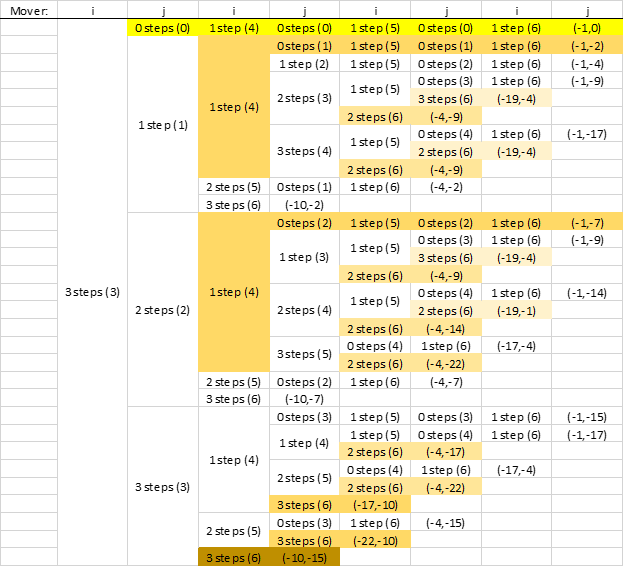
\includegraphics[scale=.5]{table4a.png}
		\end{center}
	
	We can determine the optimal play for each player using backward induction. If a player is three steps from the end, then they have current costs of -6, -9, or -15, so they will always choose to take three steps and win if any other move results in a subgame in which they lose. Thus, there is no equilibrium where a player who is three steps away from the finish line loses, and their opponent, knowing this, will minimize their losses by not taking any steps once the player reaches three steps. However, as was shown in the table below, there is no strategy in which taking three steps in one turn is preferable to losing without taking any steps. Thus, if the player who moves first takes a single step, then the player who moves second will never take three steps, and they cannot win by only moving one step. This also suggests that the player who moves first can force a win by moving two steps.
	
	Therefore, we need only determine whether the player who moves first will take one step or two. If taking one step forces a win, then their maximum payoff will come from doing so, then taking one step until the reach six. If the second-moving player responds to a one-step opening move by taking two steps, then the first-moving player can force a win by taking two steps and reaching the three-step mark. Thus, the second-moving player's best response to any first move other than 0 steps is to take 0 steps.
	
	Therefore, the unique subgame perfect equilbirium is $(1,0,1,0,1,0,1,0,1,0,1)$, which results in a payoff of $(8,0)$.
	
	\item In the absence of competition, the result is no different from in equilibirum for the winning player. This is because the winning player is minimizing costs without regard to their opponent's behavior. The losing player's behavior differs because, without competition, they would choose to take two steps at a time for six turns. However, knowing they won't get a payoff due to the other player's advantage, they choose instead to incur zero costs.
	
\end{enumerate}

%%%________________________________________________________________%%%

\subsection*{Question 5}
In a two-player game of perfect information, each player knows precisely what their payoffs, and those of their opponent, are at each terminal node (if the game is finite, every play leads to a terminal node). Further, they know what their opponent will play, either totally (i.e. as a first play or as a play in a simultaneous game) or in response to their own move. Thus, for any decision node, each player can determine their terminal payoff from any move. In a zero-sum game, one player ``wins" and the other loses at every terminal node, so the player who moves first will choose a move that enables them to win, taking into account the moves that they know they and their opponent will make, using the subgame equilibrium at each deicision node. If payoffs strictly differ across terminal nodes, then the player who moves first will choose the move that leads to the terminal node with the highest payoff. If the node with the highest payoff for the first-moving player does not have a unique payoff, then the payoff vector will be the same across all terminal nodes with that payoff for the first-moving player, since the game is zero-sum. Thus, each finite, two-player, zero-sum game with perfect information has a unique, subgame perfect equilbibrium payoff vector, though the set of moves that produces this vector is not necessarily unique.


%%%________________________________________________________________%%%

\subsection*{Question 6}

\begin{enumerate}[(a)]
	\item This game consists of two firms, ${N=\{A,B\}}$ with symmetric action sets, ${A_i=\{p_i\in\R_+\}}$, and payoff functions, ${u_i=\{p_i(D_i(p_i,p_j))\}}$. Firm $i$'s best response funciton can be found using the first-order condition of its payoff function with respect to its action, $p_i$:
		\begin{align*}
			\frac{\partial u_i}{\partial p_i} = d - 2p_i + \alpha p_j &= 0	\\
												p_i &= \frac{1}{2}d + \frac{\alpha}{2}p_j
		\end{align*}
		If both firms choose simultaneously, then, in equilibirum, each firm will input the other's best response funciton into its own and determine its action from there:
		\begin{align*}
			p_i &= \frac{1}{2}d + \frac{\alpha}{2}\left(\frac{1}{2}d + \frac{\alpha}{2}p_i\right)	\\
			\left(\frac{4-\alpha^2}{4}\right) p_i &= \left(\frac{2+\alpha}{4}\right)d 	\\
			p_i &= \left(\frac{2+\alpha}{4-\alpha^2}\right)d = \left(\frac{1}{2-\alpha}\right)d
		\end{align*}
		Thus, the symmetric Nash equilibrium is ${(p_A,p_B) = \left(\left(\frac{1}{2-\alpha}\right)d,\left(\frac{1}{2-\alpha}\right)d\right)}$.
	
	\item If firm $A$ moves first, then it knows that firm $B$ will maximize its profit according to its best response function. Thus, firm $A$'s payoff function is:
		\[
			u_A=p_A\left(d - p_A + \alpha\left(\frac{1}{2}d + \frac{\alpha}{2}p_A\right)\right) = \frac{3\alpha}{2}dp_A + \left(\frac{\alpha^2-2}{2}\right)p_A^2
		\]
		We can find the profit-maximizing price for firm $A$ using the first-order condition of its modified payoff function:
		\begin{align*}
			\frac{\partial u_A}{\partial p_A} = \frac{3\alpha}{2}d + \left(\alpha^2-2\right)p_A  &= 0	\\
			\left(\alpha^2-2\right)p_A  &= -\frac{3\alpha}{2}d	\\
			p_A &= \left(\frac{3\alpha}{4-2\alpha^2}\right)d
		\end{align*}
		Which firm $B$ will take as given, choosing $p_B$ according to its best response function:
		\begin{align*}
			p_B &= \frac{1}{2}d + \frac{\alpha}{2}\left(\frac{3\alpha}{4-2\alpha^2}\right)d	= \left(\frac{3\alpha^2}{4-2\alpha^2}+1\right)\frac{1}{2}d \\
				&= \left(\frac{\alpha^2 + 4}{2-\alpha}\right)\frac{1}{4}d 
		\end{align*}
		Thus, the subgame perfect equilibrium is ${\left(\left(\frac{3\alpha}{4-2\alpha^2}\right)d,\left(\frac{\alpha^2 + 4}{2-\alpha}\right)\frac{1}{4}d \right)}$.
		
	
	\item Letting $p_i^{sim}$ and $u_i^{sim}$ be the equilibrium price chosen and payoff earned, respectively, by $i$ under simultaneous play, with sequential play denoted without a superscript, we can solve [NOT FINISHED BELOW; am I missing a major cancellation or something? It can't actually be this messy]:
		\begin{align*}
			p_A	&= \left(\frac{3\alpha}{4-2\alpha^2}\right)d = \left(\frac{3\alpha}{2-\alpha^2}\right)\left(\frac{2-\alpha}{2}\right)\left(\frac{1}{2-\alpha}\right)d	\\
				&= \left(\frac{3\alpha}{2}\right)\left(\frac{2-\alpha}{2-\alpha^2}\right)p_A^{sim}		\\
			p_B	&= \left(\frac{\alpha^2 + 4}{2-\alpha}\right)\frac{1}{4}d  = \left(\frac{\alpha^2 + 4}{4}\right)\left(\frac{1}{2-\alpha}\right)d	\\
				&= \left(\frac{\alpha^2}{4} + 1\right)p_B^{sim}	\\
			u_A^{sim} 	&= p_A^{sim}\left(d-p_A^{sim} + \alpha p_B^{sim}\right) = \left(\frac{1}{2-\alpha}d\right)\left(d - \frac{1}{2-\alpha}d + \frac{\alpha}{2-\alpha}d\right)	\\
						&=  \left(\frac{1}{2-\alpha}d\right)^2	\\
			u_B^{sim} 	&= u_A^{sim} = \left(\frac{1}{2-\alpha}d\right)^2	\\
			u_A	&= p_A\left(d-p_A + \alpha p_B\right) 	\\
				&= \left(\frac{3\alpha}{2}\right)\left(\frac{2-\alpha}{2-\alpha^2}\right)p_A^{sim}\left(d-\left(\frac{3\alpha}{2}\right)\left(\frac{2-\alpha}{2-\alpha^2}\right)p_A^{sim} + \alpha \left(\frac{\alpha^2}{4} + 1\right)p_B^{sim}\right) \\
				&= \left(\frac{3\alpha}{2(2-\alpha^2)}\right)d\left(d-\left(\frac{3\alpha}{4-2\alpha^2}\right)d + \alpha \left(\frac{\alpha^2 + 4}{4(2-\alpha)}\right)d\right)	\\
				&= \left[\frac{1}{2-\alpha^2}-\frac{3\alpha}{2(2-\alpha^2)^2}+\alpha\left(\frac{\alpha^2 + 4}{4(2-\alpha)(2-\alpha^2)}\right)\right]\left(\frac{3\alpha}{2}\right)d^2	\\
			u_B &= \left[1-\frac{\alpha^2+4}{4(2-\alpha)} + \alpha\left(\frac{3\alpha}{2(2-\alpha^2)}\right)\right]\left(\frac{\alpha^2+4}{4(2-\alpha)}\right)d^2
		\end{align*}
	
	
\end{enumerate}


%%%________________________________________________________________%%%


\end{document}




































